%!TEX root = ../../super_main.tex

\section{Multi project organization}

This semester project is the continuation of a widely spanning multi project with 52 developers which are organized in 14 smaller groups, up to four developers per group, including a group consisting of the authors of this report. The multi project was split into 3 different project areas: Build and Deployment, GUI, Database. 

\subsection{Organization}
The multi project was organized using the development method Scrum\parencite{scrum}, more specific Scrum of Scrums. This method alows the multiproject to be self-organized and enforces the individual groups to do work more independetly. This independent work fits great in since the individual groups is used to work in smaller projects groups. However in this semetester the groups will now obtain experience in working on a larger scale projects than previous encountered in their education. 
\\\\
As seen in \figref{fig:scrum_of_scrums} the Scrum of Scrums is split into three levels. The bottom most level is the individual groups, which work exactly as an ordinary development group using the Scrum method. The middle layer contains the three project areas where representatives from each individual group meet and syncronize their work at least twice a week. The top layer in \figref{fig:scrum_of_scrums} contains representatives from all of the project areas. However since standup meeting only occur once a week in this Scrum representatives from all groups are encouraged to join the meetings.

\todo[inline]{Update Figure}
\begin{figure}[!htbp]
  \centering
    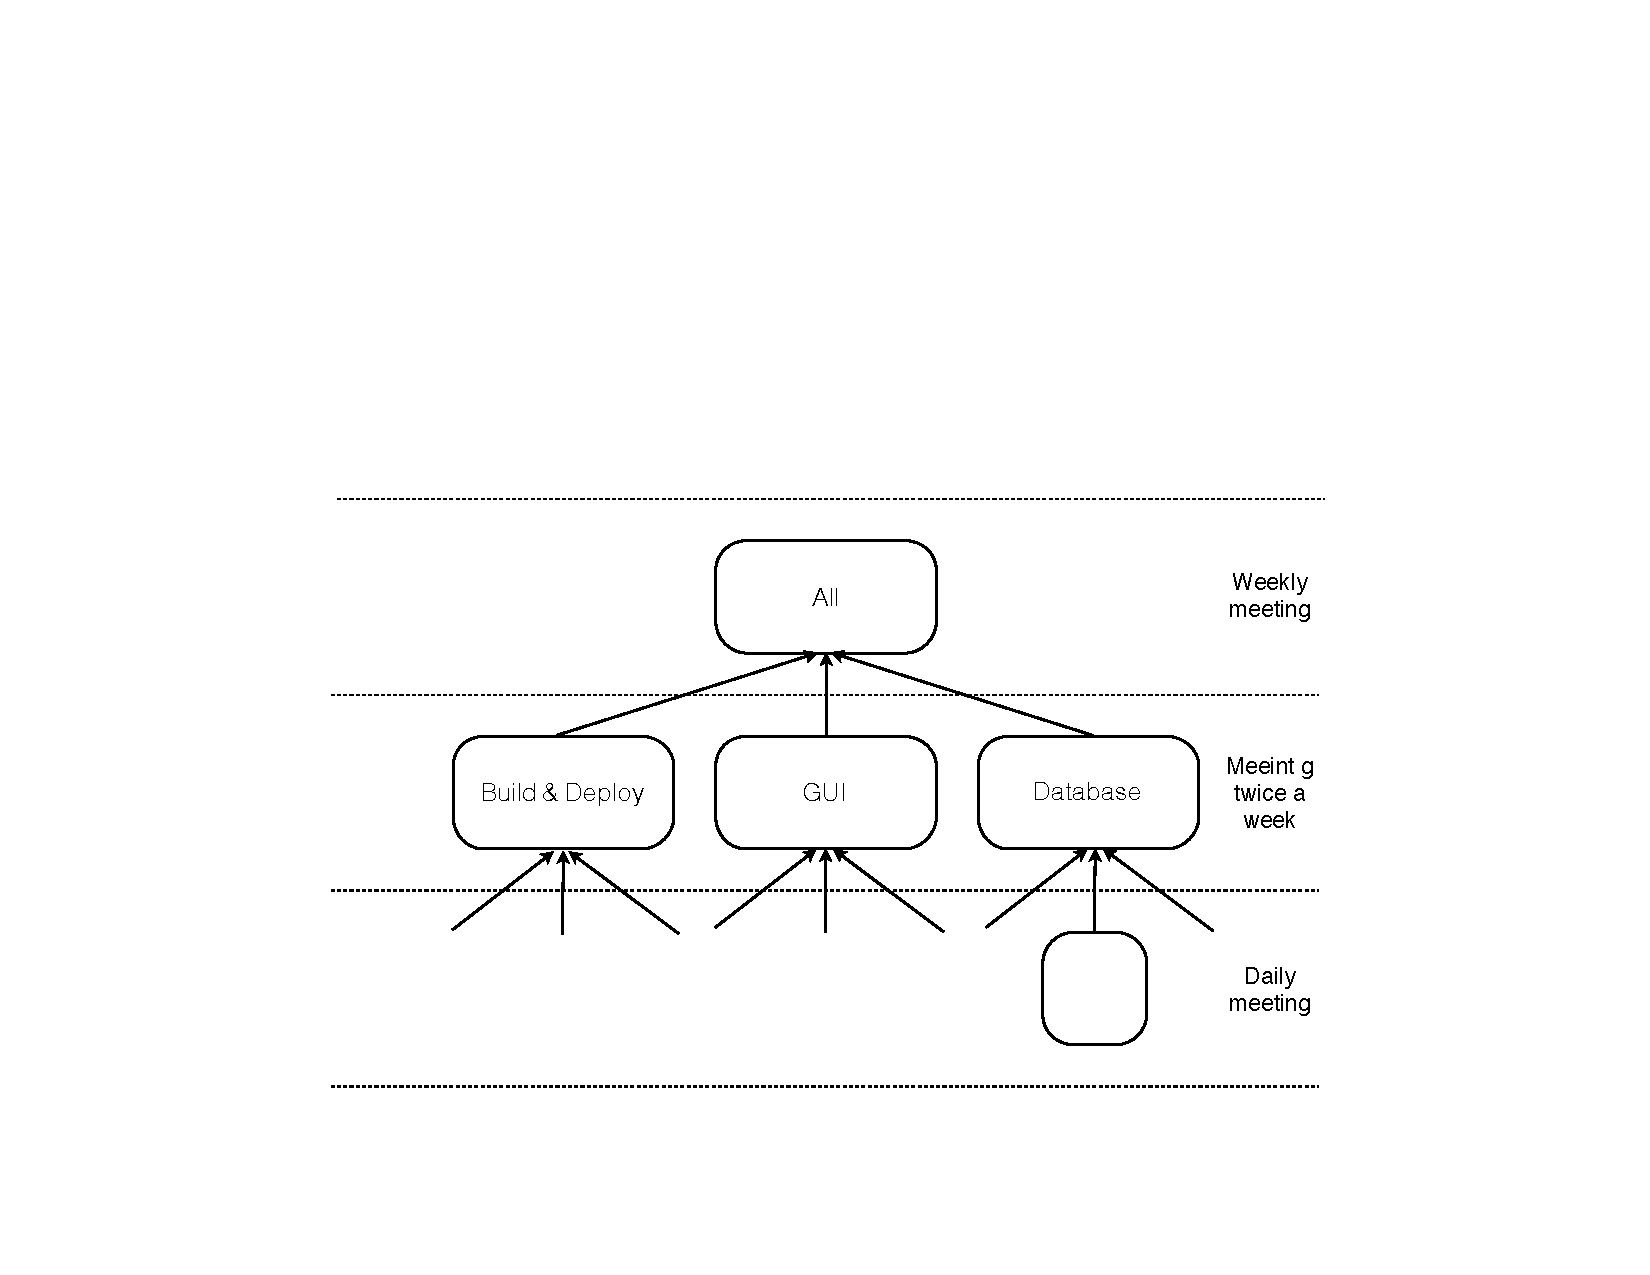
\includegraphics[width=0.6\textwidth]{scrum_of_scrums}
    \caption{Organization in Scrum of Scrums.}
    \label{fig:scrum_of_scrums}
\end{figure}



\subsection{Roles and Responsibilities}
Several different roles and responsibilities were divided among the project groups. This group volunteered as ``Webadmin'' and also included an Android Guru. The ``Webadmin'' responsibility included administration of the official \giraf web page. The android guru responsibility included helping out with Android related issues that groups could not handle within reasonable time themselves and setting up a general Android guideline. 